%Headers
% for old version
%\documentstyle[epsbox,fancyhdr,indent,a4j,10pt]{jarticle}          % use this for preprint style
% for 2e version
\documentclass[a4j,10pt]{jarticle}
\usepackage{graphicx, epsbox,fancyhdr,indent}

%\nonstopmode

%\setlength{\oddsidemargin}{-1cm}
%\setlength{\evensidemargin}{-1cm}
\setlength{\textwidth}{5.5in}
\setlength{\headheight}{15.0pt}

\pagestyle{fancyplain}
\addtolength{\headwidth}{\marginparsep}
\addtolength{\headwidth}{\marginparwidth}
\lhead[\fancyplain{}{\bfseries\thepage}]%
       {\fancyplain{}{\bfseries\rightmark}}
\rhead[\fancyplain{}{\bfseries\leftmark}]%
       {\fancyplain{}{\bfseries\thepage}}
\cfoot{}

\renewcommand{\topfraction}{.8}
\renewcommand{\textfraction}{.1}
\renewcommand{\floatpagefraction}{.8}
\setlength{\textheight}{23cm}

\usepackage{maple2e}
 \def\emptyline{\vspace{12pt}}
\DefineParaStyle{Maple Output}
\DefineParaStyle{Maple Plot}
\DefineParaStyle{Warning}
\DefineCharStyle{2D Math}
\DefineCharStyle{2D Output}

\begin{document}
\title{核生成理論における平衡自由エネルギー}
\author{関西学院大学・理工学部・情報科学科 西谷滋人 
}

\maketitle

\section{Introduction}
我々が最近提案した析出核の自由エネルギー変化の精密計算法は,核生成の自由エネルギーをエンタルピー項とエントロピー項に分け,前者を第一原理計算によって,後者を統計熱力学からの見積もりによって精確に計算する.

この研究の動機は,藤田英一阪大名誉教授の「核生成にはエネルギーバリアがない」という主旨の論文,発表で,私自身が理解している範囲で藤田ジレンマについて先ずまとめておく.西谷は先の研究で藤田ジレンマに対する一応の解答を得たと考えている.

藤田自身の問題意識は,30年以上にわたってこの問題を発信してきたことからも分かる通り,それを理解するととても深く,示唆に富んでいる.しかし,その「核生成にはエネルギーバリアがない」とか「不足分が本体分を越す」などといった禅問答のような表現が独り歩きしている.これはセンセーションを狙った藤田特有の物言いで,翁のおちゃめと解している.しかしその示唆は貴重で,1973年の論文中\cite{Fujita:1973}の「反応速度式の考え方と,前述の核形成論とを結びつけるようなやり方」として出された読者への宿題を本気で解いていれば,\cite{BinderStauffer:1976}の有名なクラスターダイナミックスに先んじていたかもしれない.

\section{核生成理論のどこが議論されているか(藤田論文の波紋)}
まず古典的核生成論は,材料の多くの教科書に出てくるとおり,相転移において新相のエンブリオが核として成長する前段階では系のエネルギーは正となり,それを超えるための活性化過程があるとする.エンブリオを半径$r$の球状として,そのエネルギーを表現する式,
\begin{equation}
\Delta G = -\frac{4}{3}\pi r^3 \epsilon + 4 \pi r^2 \gamma
\label{Eq:1}
\end{equation}
において,$r$が小さいと$r^2$を含む表面エネルギー$\gamma$による右辺第二項が$r^3$を含む体積エネルギー$\epsilon$による第一項を優先し,図\ref{NucleationFreeE}に示すように,成長初期には$\Delta G$が上昇し,臨界寸法と臨界エネルギーが現れ,したがって核生成は活性化過程をともなうとする.
\begin{figure}[ht]\begin{center}
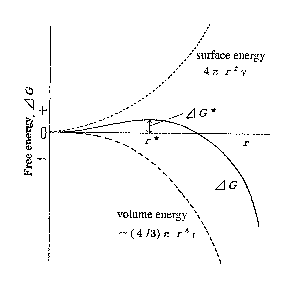
\includegraphics[width=65mm]{./figs/NucleationFreeE.eps}
\caption{核生成の自由エネルギー変化の模式図.}
\label{NucleationFreeE}
\end{center}\end{figure}

これに対する藤田の批判は以下の通りである\cite{Fujita:2003}.「第一に,表面(界面)エネルギーの本性は,原子集団の凝集エネルギーの表面における不足分に大部分由来すると考えられる.すなわち図\ref{SurfaceEnergy}に示したように,孤立した原子集団の内部の原子がまわりの原子群と十分な結合状態を持つのに対して,表面原子は結合相手が約半分しかなく,したがって相手の数が不足して結合エネルギーの下がりが不十分であり,破線で示したこの不足分(欠損分)を完全な結合状態からの上がり分,即ち,正の値を持つ表面エネルギーとして別個に考えているのである.通常,これを抜き出して,点線のように表面の位置に突出したエネルギー分として描くが,この山は長い曲がった矢印が示すように,破線に当たる結合状態からの立ち上がりでなくてはならない.したがって,(\ref{Eq:1})式の第二項が第一項に優るならば,不足分が本体分を越すという矛盾になるであろう.」
\begin{figure}[ht]\begin{center}
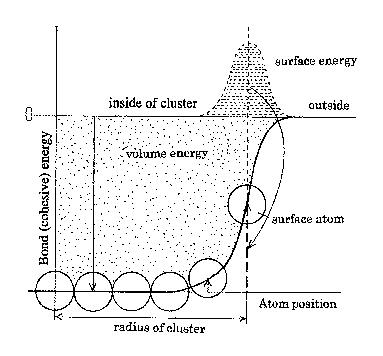
\includegraphics[width=65mm]{./figs/SurfaceEnergy.eps}
\caption{表面エネルギーの概念図.}
\label{SurfaceEnergy}
\end{center}\end{figure}

さらに,「2原子分子的な結合,即ちdimer,あるいは3原子集合のtrimerその他の小さな集合体は実際に存在し,それらの結合は常に引力的とせざるを得ず,小さい集団では正のエネルギーを持つとは考えられていない.」という例を出している.これらの考察は,「表面(界面)エネルギーのせいで自由エネルギーが正になるわけがない」,あるいは「結合エネルギーの変化だけを考えると,山はできな」ということを示唆している.

また駆動力については,その著書(\cite{Fujita:1996})のなかで指摘している.図\ref{Precipitation}の析出過程では,高温での均質固溶領域から時効温度($T_a$)へ系が持ちきたらされたときの自由エネルギー変化に対応している.すなわち,自由エネルギーの変化は図\ref{DrivingForce}にしめすような組成自由エネルギー曲線を考える.系全体の自由エネルギー変化はoからuへの変化である.しかし,これが駆動力になるわけではない.駆動力は,初期組成$c_0$での自由エネルギー曲線の接線の延長qから,析出物の自由エネルギーsへのエネルギー差に相当する.そこでは化学ポテンシャルという言葉が用いられているが,これは一原子の持っている自由エネルギーと考えれば理解されよう.
\begin{figure}[ht]\begin{center}
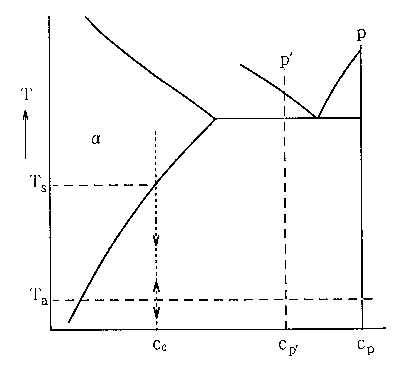
\includegraphics[width=65mm]{./figs/Precipitation.eps}
\caption{析出処理.}
\label{Precipitation}
\end{center}\end{figure}
\begin{figure}[ht]\begin{center}
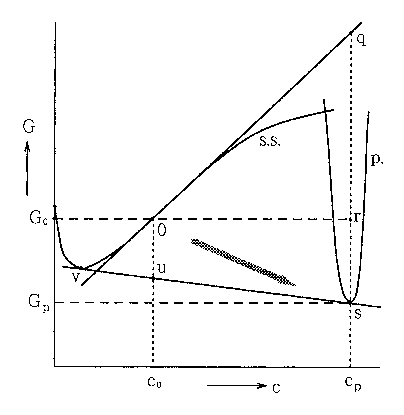
\includegraphics[width=65mm]{./figs/DrivingForce.eps}
\caption{析出にともなう自由エネルギー変化.}
\label{DrivingForce}
\end{center}\end{figure}

これらの指摘は正しい.また,\cite{Fujita:2003}ではさらに,活性化の要因となる,歪エネルギー,振動エネルギーの効果も挙げている.しかし,これらの影響がない場合に,すなわち配置の変化にともなうエンタルピー,エントロピーの変化だけで活性化の山は出るのであろうか? さらに,藤田の指摘以外にも核生成自由エネルギーを表す図\ref{NucleationFreeE}には謎がある:(i)なぜクラスターサイズ$n$の関数なのか,(ii)そもそもこの図の縦軸の原点はなになのか? これらの問題を考える前に,現在受け入れられている核生成理論において,この自由エネルギーはどのように扱われているかを見ておく必要がある.

Appendix Aには\cite{BeckerDoring:1935}の取り扱いをまとめている.ここで重要な点は,dropletモデルの自由エネルギーはclusterの反応係数の導出で,detailed balanceが成り立つためにしか用いられていない点である.また,Appendix BにはLanger(\cite{Langer:1967,Langer:1969}のgrand partition functionの導き方を示した.ここでも,自由エネルギーはexcess energyとして使われているだけである.つまり,どちらのより厳密な核生成理論も,自由エネルギーをクラスターサイズあるいは溶質原子$n$個に限られたcanonical ensembleとして使われている.こうなると,自由エネルギーの横軸がなぜ,$n$のあるいは$r$の関数となるかが理解されよう.つまり,溶質の原子数を固定したcanonical ensembleで自由エネルギーを計算すればいいことが示唆される.このような理解にたって,我々の核生成自由エネルギーの第一原理計算を見ていこう.藤田の疑問はその中で明らかとなる.
\iffalse
\subsection{Stowellの解析}
StowellはKashchievの関係を使ってCu-Co合金について詳しい解析をおこなっている.定常状態の核生成速度$J$と潜伏時間$\tau$は今まで得られた式を書き直すと
\begin{eqnarray}
J&=&Z\beta C(n^*) \\
\tau &=& (\theta \beta Z^2)^{-1}
\end{eqnarray}
である.Kashchievはこの積$J\tau$が理論の正当性を直接測る重要な値であることを指摘した.積を取ると
\begin{equation}
J\tau = C(n^*)/\theta Z
\end{equation}
となり,動力学係数$\beta$が消える.$\theta$は1に近い定数と期待でき,また$Z$も通常0.1程度の定数であるので,この積はクラスター密度の$C(n^*)$の直接的な指針となると考えられる.これを界面エネルギー用いた古典的な取り扱いから
\begin{equation}
\ln(J\tau) = \ln(N_0/\theta Z) - (16 \pi \sigma^3 \nu_{\rm b}^3/3k^2/[ T^3(\ln S)^2 ]
\end{equation}
を導出している.LeGouesとAaronsonによって得られた実験結果をうまく解釈するには至っていない.しかし,これは我々の新しい手法によって臨界核が十分に小さければ直接第一原理計算から出すことが可能かもしれない.

\section{界面エネルギーの取り扱いやこれから勉強すべき内容のメモ}
\subsection{エントロピー効果}
H.I.Aaronson, J.B.Clark, and C.Laird
Metal Science Journal, 2(1968), 155--158
M.Sluiter and Y.Kawazoe, 54(1996), 10381--10384.
\subsubsection{離散格子モデル}
\subsubsection{Cahn-Hilliardモデル}
\section{核生成の平衡自由エネルギーのいろいろ}
Reiss and Bowless\cite{ReissBowles99}の指摘は上記のeq.1式において定義される$n$分子を含んだクラスターの平衡平均個数$\bar{\nu}(n)$が
\begin{equation}
\bar{\nu}(n) = \bar{\nu}(n) \exp\left(-W/kT\right)
\end{equation}
で与えられるという式の根拠を怪しんでいる.ここで$W$は$n-$クラスターを形成する可逆仕事を意味している(このあたりの用語は化学の分野では普通か?).

\subsection{Drossinos and Kevrekidis}
ほぼ同じ問題提起が2003年にDrossinos and Kevrekidis \cite{DrossinosKevrekidis03}によってなされている.彼らの指摘通り,この問題は1960年代にLothe-Poundによってtranslation-rotation paradoxとして取り上げられている.Lothe-Poundを引き継いだFederら\cite{Feder66}によると,この問題はKuhrtによって\cite{Kuhrt52}1952年に初めて取り上げられたらしい.

Dillmann and Meier\cite{DillmannMeier91}がまとめている(16)式に長年にわたる議論の結果が凝集している.一個の$n-$クラスターに対する自由エネルギーは
\begin{equation}
\beta \Delta \Omega(n) = -n \ln S + k_N \sigma n^{2/3} +
\tau \ln n - \ln(q_0 V)
\end{equation}
とまとめられる.ここで$S$はsuper saturation ratio(例えば$p_e/p$),$k_N$はクラスター表面エネルギーのマクロな液滴からの$N$個の独立な"ふれ"を意味する.一方,$\tau, q_0$は可変パラメータである.最初の2項は古典的なモデルでの体積項と表面項を表し,後ろの2項が位置および配置のエントロピーを表している.

この式はFisher\cite{Fisher65,Fisher67}によってまとめられたdropletモデルをもとに,Dillmann and Meier\cite{DillmannMeier91}が精巧に再構築した.$\tau = 0$が古典的なDropletモデルに対応する.$\tau$の依存性はDillmann and Meierで詳しく論じられているが,面白いのはこの値は理論的に確定しているわけではなさそうなところである.

\subsection{平衡クラスター分布に関するFederらによる記述\cite{Feder66}}
サイズ$n$の全てのクラスターは単位体積あたり,
\begin{equation}
F_n = c(n) f_n -c(n)kT \ln \frac{e}{c(n)}
\end{equation}
というHelmholtzの自由エネルギーを持ったsub-systemを形成する.一個のクラスターの単位体積あたりの自由エネルギーを$f_n$とする.これにはクラスターの並行移動(translation)あるいは回転(rotation)の自由エネルギーも含まれる.
\subsection{Lothe and Pound}
A much more contribution arises from further consideration of the absolute entropy of the embryos or nuclei.  The translational and rotational components of the free energy of formation are given by 

respectively.  In the case of homogeneous nucleation of water droplets from vapor at 300K (i*~100), $DG_{trans}$=-24.4kT, and $DG_{rot}$=-20.8kT.
これらのentropyはまわりの原子からの拘束を考えない,vapor中のdropletでなされたものである.したがって,自由エネルギーへの寄与はやたらと大きくなっている.しかし,固体中の析出の場合にこれほど大きくなるかどうかは実際に計算する必要がある.
F. Kuhrtは1952にすでに同様の議論を行なっている.Z. Physik, 131(1952), 185--204.ドイツ語故,ちゃんとは読んでいない.
\fi
\section{析出核のエントロピー変化}
\subsection{新しい計算法の概略}
前節の考察にあるとおり,核生成の自由エネルギー変化は溶質原子数を固定して考えればいい.新しい核生成自由エネルギーの計算法は,核生成の始状態と終状態を図\ref{directMethod}のように単純に考えることに相当する.始状態は孤立・分散した溶質原子が溶媒原子中にばらばらに浮いている状態であり,終状態はサイズ$n$のクラスターを1個作った状態である.この二つの状態のエンタルピー,エントロピー変化をそれぞれ計算することによって核生成の自由エネルギーを求めることが出来る.
\begin{figure}\begin{center}
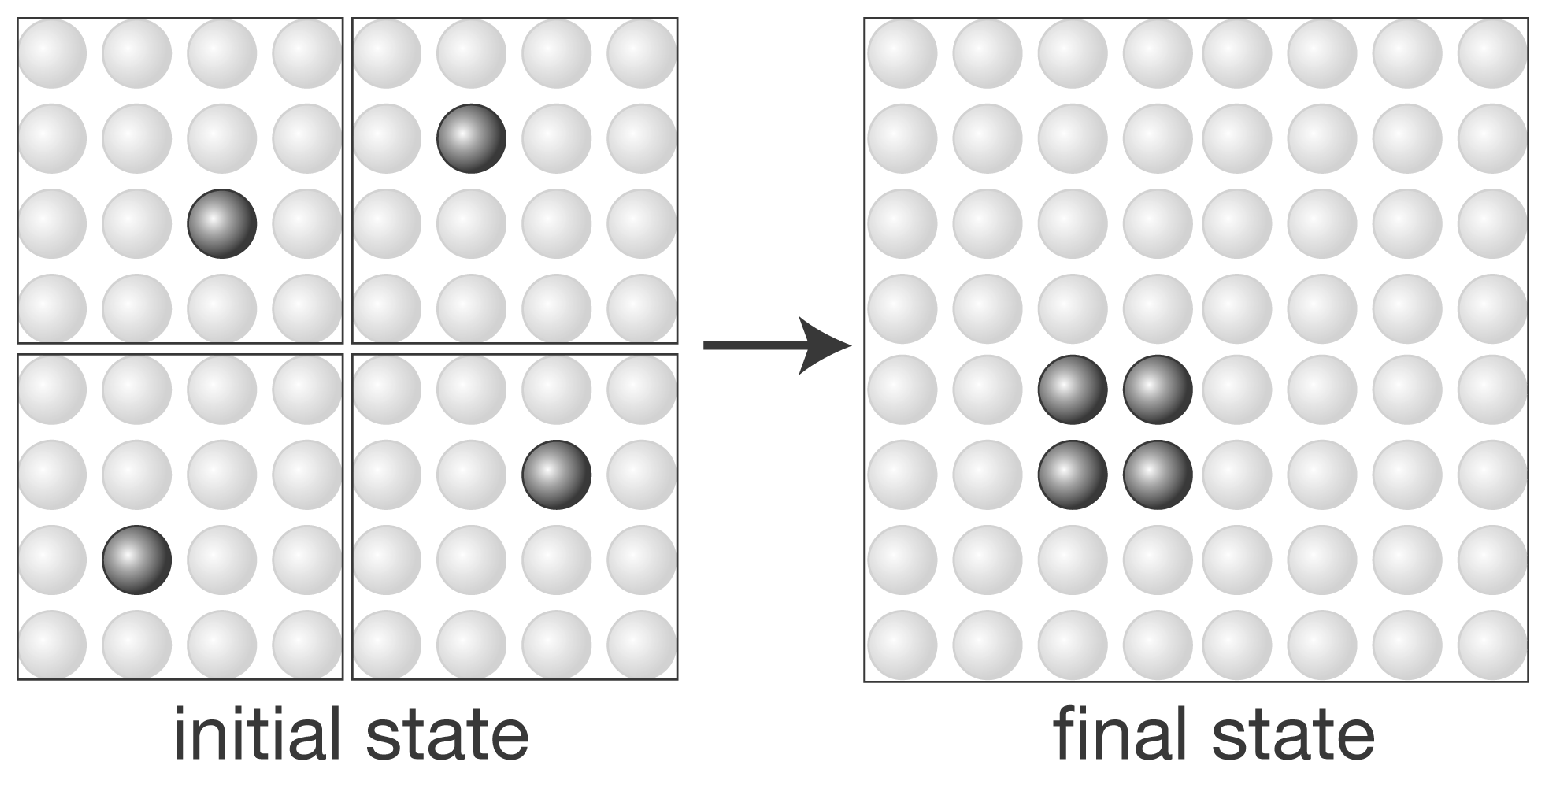
\includegraphics[width=75mm]{./figs/Fig2.eps}
\caption{核生成の始状態,終状態の模式図.}
\label{directMethod}
\end{center}\end{figure}

別の見方をすると以下のようになる.自由エネルギー$\Delta G$を
\begin{equation}
\Delta G = \left(\Delta H_{\rm V} + H_{\rm surface} \right) - T \Delta S
\label{Eq1}
\end{equation}
のようにエネルギー項とエントロピー項$S$に分ける.前者は内部エンタルピーの変化$\Delta H_{\rm V}$と界面エネルギー$H_{\rm surface}$を含んでおり,密度汎関数理論にもとづいた精密計算が可能である.後者は単純な理想溶体近似によって, $x$を初期溶質濃度とすると
\begin{equation}
\Delta S = k_{\rm B} (n-1) \ln(x)
\label{Eq2}
\end{equation}
と見積もられる\cite{KamijoFukutomi:1983}.

モデル計算をbccFe中のbccCuの析出でおこなった.第一原理計算にはVASPを用いた.bccFeとbccCuでは格子歪エネルギーは0.02eV/atomであるので,これを無視した.bccFeの一部のサイトをCu原子に置き換えてクラスターエネルギーを計算した.ここには,Cu原子同士の結合生成にともなうエネルギー変化と界面のFe-Cu原子間の結合による界面エネルギーとが含まれている.図\ref{ClusterEnergy}はsegregation limitから測ったクラスターエネルギーである.(\ref{Eq1})式のエネルギー変化は孤立した溶質原子エネルギー(dilution limit)からのズレであるので,図\ref{ClusterEnergy}の直線からの差がこれに相当する.これに(\ref{Eq2})式のエントロピー変化を加えると図\ref{ClusterFreeEnergy}のようなクラスター生成自由エネルギー変化が得られる.Fittingによって求めた臨界半径や活性化エネルギーはそれぞれ10-25個,0.4-0.8eVであった.これらはGoodmanら\cite{Goodman:1973b}が理論的に推測し,その後の実験の解釈に用いられている値と一致している.

\begin{figure}\begin{center}
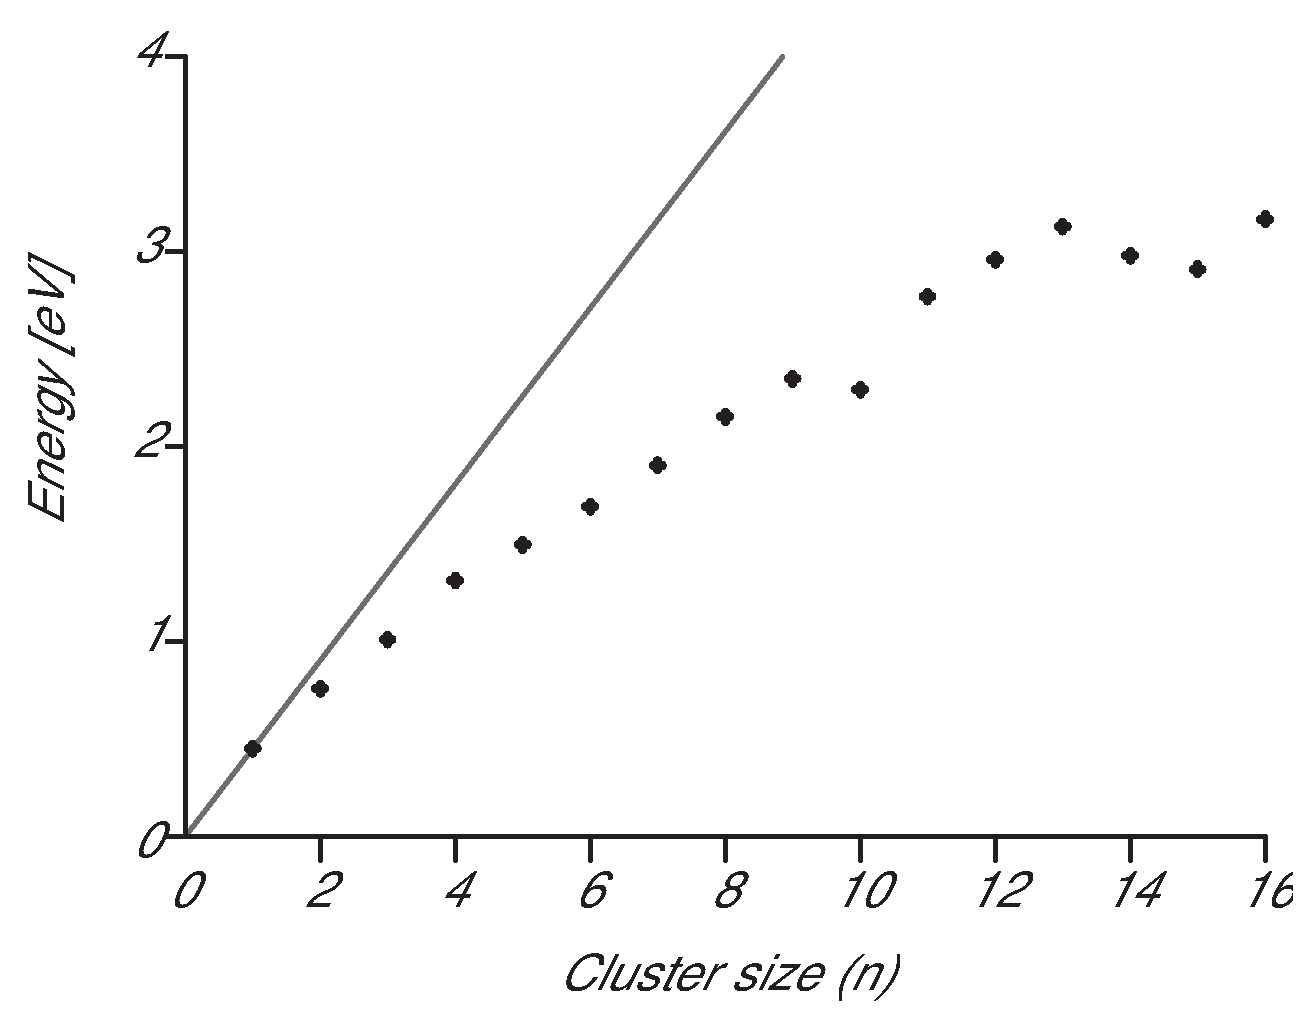
\includegraphics[width=75mm]{./figs/ClusterEnergy.eps}
\caption{クラスターエネルギーのサイズ依存.}
\label{ClusterEnergy}
\end{center}\end{figure}
\begin{figure}\begin{center}
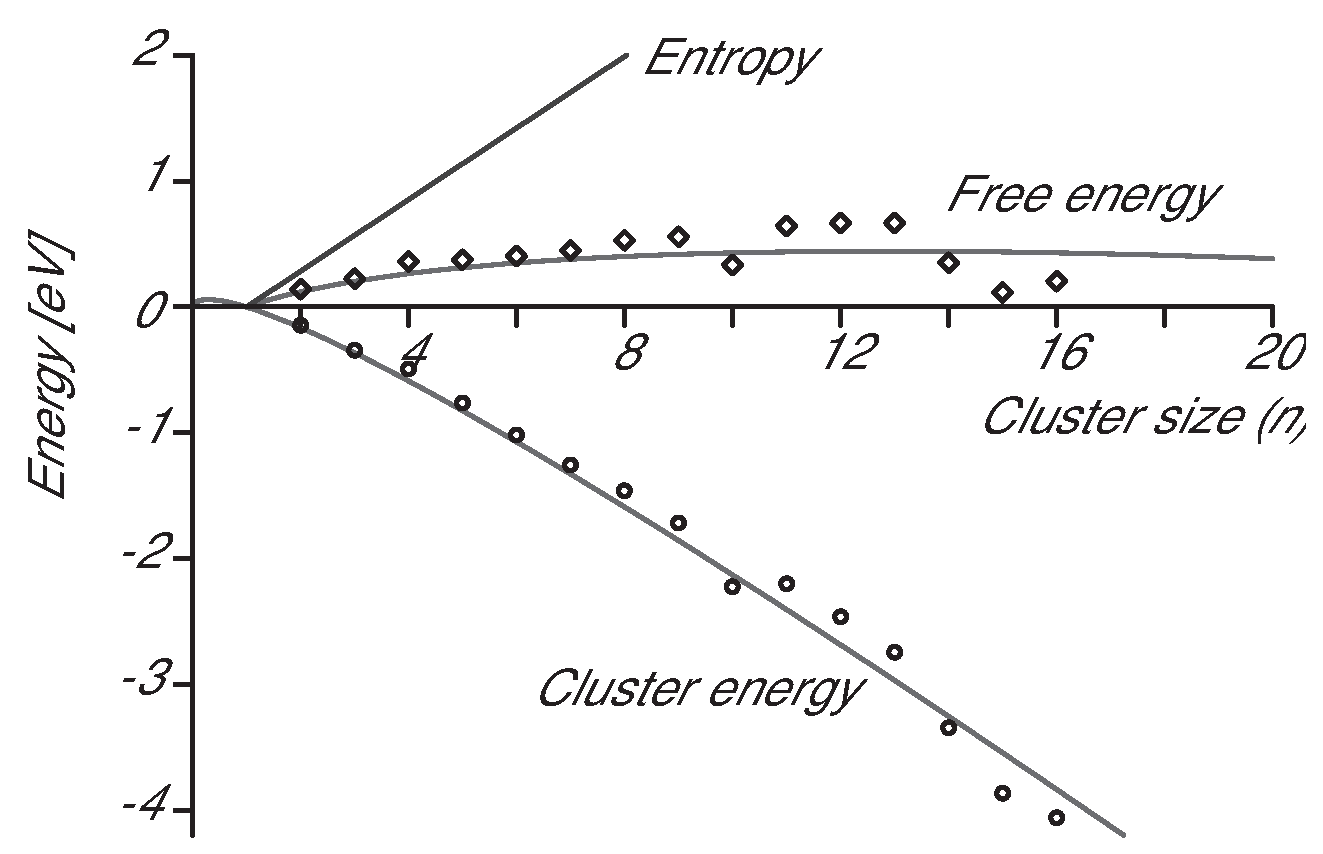
\includegraphics[width=75mm]{./figs/ClusterFreeEnergy.eps}
\caption{クラスターの自由エネルギー変化.}
\label{ClusterFreeEnergy}
\end{center}\end{figure}

藤田が考えていたボンドの変化によるエネルギー変化は,ここではcluster energyに相当する.そこでは確かに山は存在せず,単調減少する関数となっている.また,自由エネルギーの図の原点がdilution limitにあることが分かる.つまり溶質原子が一個ある状態が,お互いに相互作用せずに何個もある状態を考える.これは初期組成の自由エネルギーの接線の延長に相当する.このモデルでは,初期組成,温度の影響はすべてエントロピー項の傾きに押し込められている.これらの過飽和度の変化に連れて活性化の山は移る.また,このような絶妙なエントロピーの値を見積もるのは一般的なモデルでは難しく,このあたりの影響を藤田が見誤ったのではないかと推測される.
%\iffalse
\subsection{エントロピー変化(並進)}
前節に示した通り,析出核生成に伴う自由エネルギー変化のなかで,エンタルピー変化は第一原理計算法によって適切に扱うことが可能である.そこでは,比べるべき,始状態と終状態が明確に定義されている.では,エントロピーはどうであろうか?

前節の取り扱いではエントロピー変化は単純なBragg-Williams近似が成り立つと仮定した.しかし,実際のエントロピー変化は,より精確に場合の数を数える必要がある.析出核の形状として球形を仮定した場合には場合の数が発生しないが,多原子分子クラスターが高温で回転の自由度を持つように,回転にともなう場合の数が発生することが期待される.図\ref{SchemRotation}にこの様子を模式的に示した.ある形状のクラスターがとる配置は,代表点(中心)を決めると,その並進とそのまわりの回転の単純な積である.クラスターがとる場合の数は,
\begin{equation}
W = W_{\rm trans} \times W_{\rm rot}
\end{equation}
となる.先ずは並進にともなうエントロピー変化の導出を示す\cite[小田垣卒論]{Odagaki03}.

\begin{figure}\begin{center}
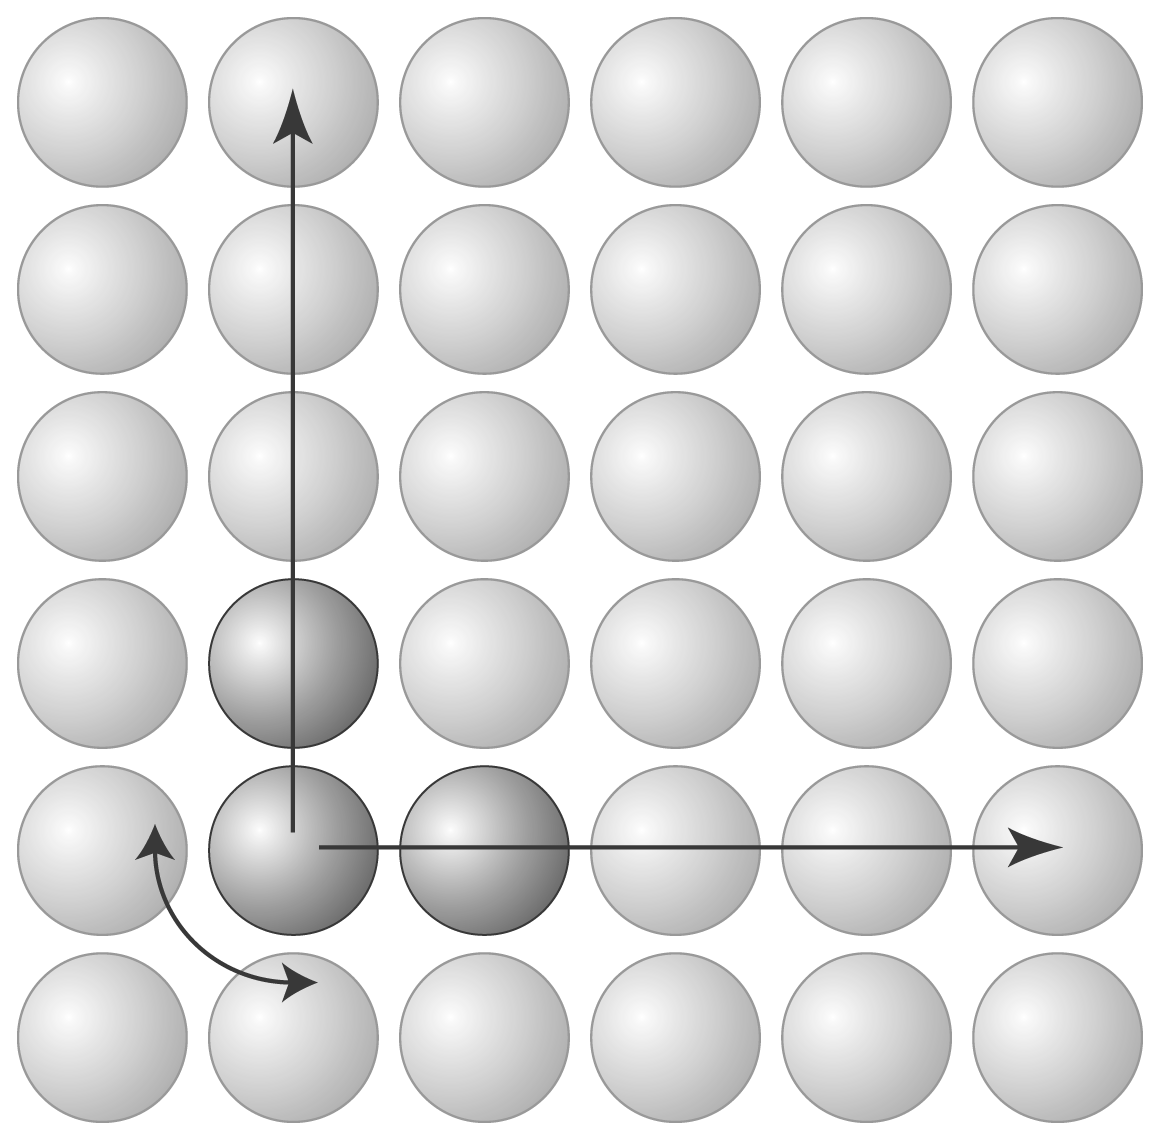
\includegraphics[width=35mm]{./figs/SchemRotation2.eps}
\caption{クラスターの場合の数.}
\label{SchemRotation}
\end{center}\end{figure}

核生成前後の配置の場合の数からエントロピー変化の導出を考える.2元系においてクラスターサイズを$n$原子,溶質濃度を$x$とおく.核生成に関わる領域$M$を$M = n/x$原子と定義する.溶質原子の数は$Mx$,母相原子の数は$M(1-x)$である.よって核生成前の場合数$W_{1}$は
\begin{equation}
W_{1}=\frac{M!}{(Mx)![M(1-x)]!}
\vspace{.5cm}
\label{eq:W1-binary}
\end{equation}
である.一方,核生成後の場合の数$W_{2}$はクラスター1個とFe原子$M(1-x)$個の配置を考えて
\begin{equation}
W_{2} = \frac{[M(1-x)+1]!}{[M(1-x)]!}
\vspace{.5cm}
\label{eq:W2-binary}
\end{equation}
である.クラスター内部はすべてCu原子なので場合の数は発生しない.配置のエントロピーの定義より
\begin{eqnarray}
\Delta S_\mathrm{V} &=& k_\mathrm{B} (\ln W_{2} - \ln W_{1}) \nonumber \\
&=& k_\mathrm{B} \ln \frac{[M(1-x)+1]!(Mx)!}{M!}
\vspace{.5cm}
\label{eq:S-binary}
\end{eqnarray}
を得る.式中$k_\mathrm{B}$はBoltzmann定数である.溶質が希薄かつ$M$が大きい極限ではこの式は2元系理想溶体での近似式
\begin{equation}
\Delta S_\mathrm{V} = k_\mathrm{B} ( n - 1 ) \ln (x) 
\vspace{.5cm}
\label{eq:S-kamijo}
\end{equation}
と一致する.(\ref{eq:S-kamijo})式は理想溶体の混合の自由エネルギーからエントロピー変化の式を導き,クラスターの組成を1としたときの極限である.
\subsection{回転エントロピー}
では回転の場合の数はどうやって求めればいいか.もっとも単純には格子の点対称性が最大数になることが分かる.例えば,先程の2次元正方格子では4が最大数である.bcc格子ではこれが24になる.しかし,クラスター形状自身の対称性からこの数は下がる.前節で求めた最もエネルギーの低いクラスターの形状を図\ref{ClusterConfig}にまとめた.また,それぞれのクラスターに対応する回転の場合の数を表\ref{Table:rotation}にまとめた.
\begin{figure}\begin{center}
\includegraphics[width=95mm]{./figs/cluster2.eps}
\caption{クラスターの配置.}
\label{ClusterConfig}
\end{center}\end{figure}

\begin{table}
\begin{center}
\caption[]{それぞれのクラスターにおける場合の数$W$.場合の数はaxis x rotation / symmetryで求めた.}
\label{Table:rotation}
\begin{tabular}{ccccccc}
\hline
cluster&axis&rotation&symmetry&$W$&Non-relaxed&Relaxed\\
 size($n$)&& ($\times$) & ($/$) & ($=$) &[eV]&[eV]\\ \hline
2&8&1&8&1&  -.144 &  -.163 \\
3&6&4&2(?)&12&  -.344 &  -.358 \\
4&6&4&8(?)&3&  -.493 &  -.563 \\
5&6&4&2&12&  -.763 &  -.952 \\
6&6&1&2&3& -1.017 & -1.162 \\
7&6&4&1&24& -1.257 & -1.432 \\
8&6&4&2&12& -1.46  & -1.658 \\
9&6&4&1&24& -1.717 & -1.964 \\
10&6&4&2&12& -2.224 & -2.227 \\
11&6&4&1&24& -2.199 & -2.512 \\
12&6&4&1&24& -2.462 & -2.818 \\
13&6&4&1&24& -2.744 & -3.127 \\
14&6&4&1&24& -3.345 & -3.728 \\
15&1&1&1&1& -3.865 & -4.271 \\
16&6&4&1&24&    & -4.511 \\
\hline
\end{tabular}
\end{center}
\end{table}%

\subsection{実際のエントロピー変化が与える影響}
図\ref{EntropyRev}には並進,回転の場合の数を含めた場合のエントロピー変化を示した.W(BW)が前節で示した単純なBragg-Williams近似を用いた場合のエントロピー変化を示す.W(BW)+W(rot24)はこれに回転の最大の場合の数(24)を加えた場合の変化,W(Trans)+W(rot24)はさらに並進の場合の数を精確に求めた場合のエントロピー変化を示す.回転の場合の数をそれぞれのクラスターの配置を考慮して求めた結果は点で示してある.これより回転の場合の数が与えるエントロピーへの影響はわずかな平行移動でしかないことが分かる(\verb"x:=0.014;k:=0.8617*10^(-4);T:=273+500;ではk*T*ln(24)=0.21eV程度").それよりも並進のスターリング近似を用いる影響が大きいことが分かる.
\begin{figure}\begin{center}
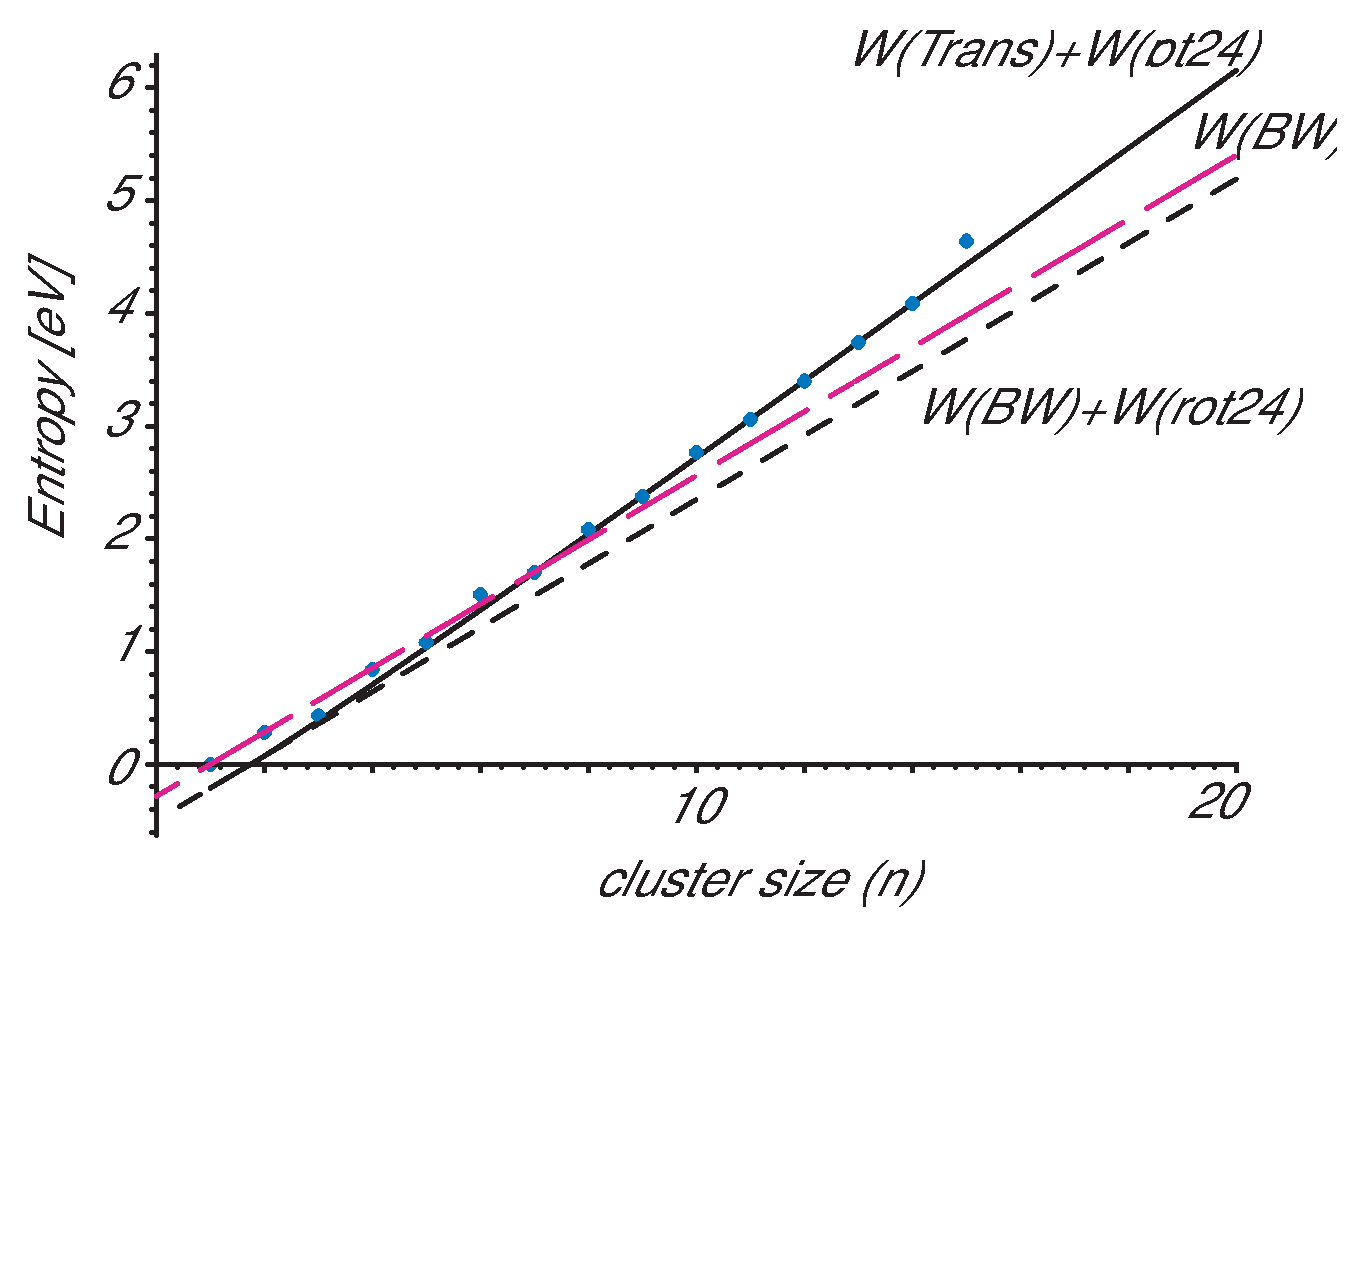
\includegraphics[width=95mm]{./figs/EntropyRev.eps}
\caption{並進,回転の場合の数を含めた場合のエントロピー変化.}
\label{EntropyRev}
\end{center}\end{figure}

さらにエンタルピー変化を加えて求めた自由エネルギー変化は図\ref{FreeEnergyRev}のようである.回転の場合の数の違いによりクラスターごとのばらつきは大きくなっている.しかし,それよりも並進の場合の数の影響で全体の傾向が右肩上がりとなり,$n=15$においても自由エネルギーが下がり始めているのか疑わしくなっている.
\begin{figure}\begin{center}
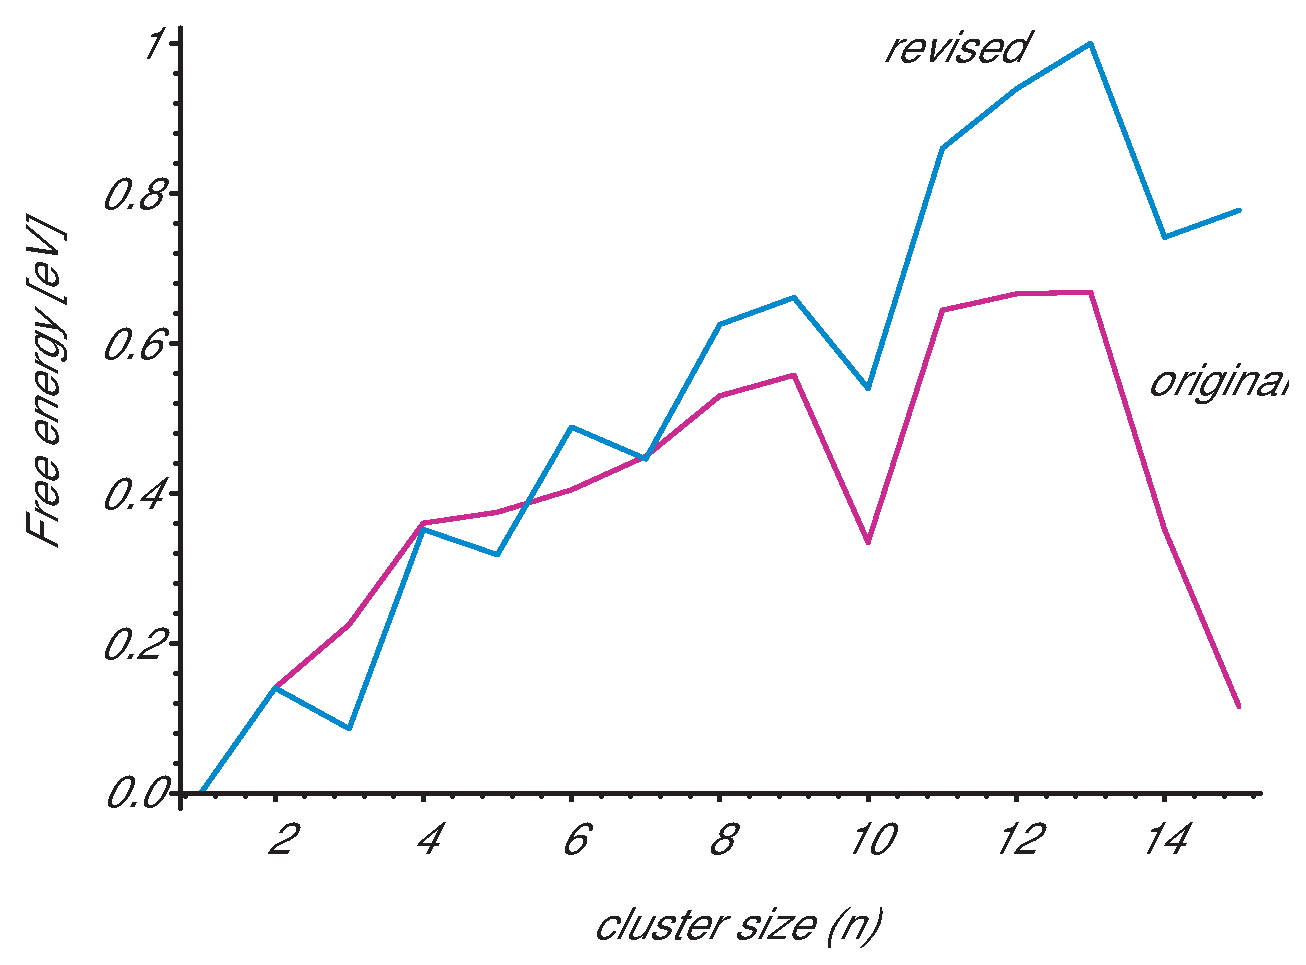
\includegraphics[width=95mm]{./figs/FreeEnergyRev.eps}
\caption{並進,回転のエントロピーを精密に求めた場合の自由エネルギーの変化.}
\label{FreeEnergyRev}
\end{center}\end{figure}

さらにエンタルピー変化としてrelaxation後の値を加えて求めた自由エネルギー変化は図\ref{FreeEnergyRev2}のようである.
\begin{figure}\begin{center}
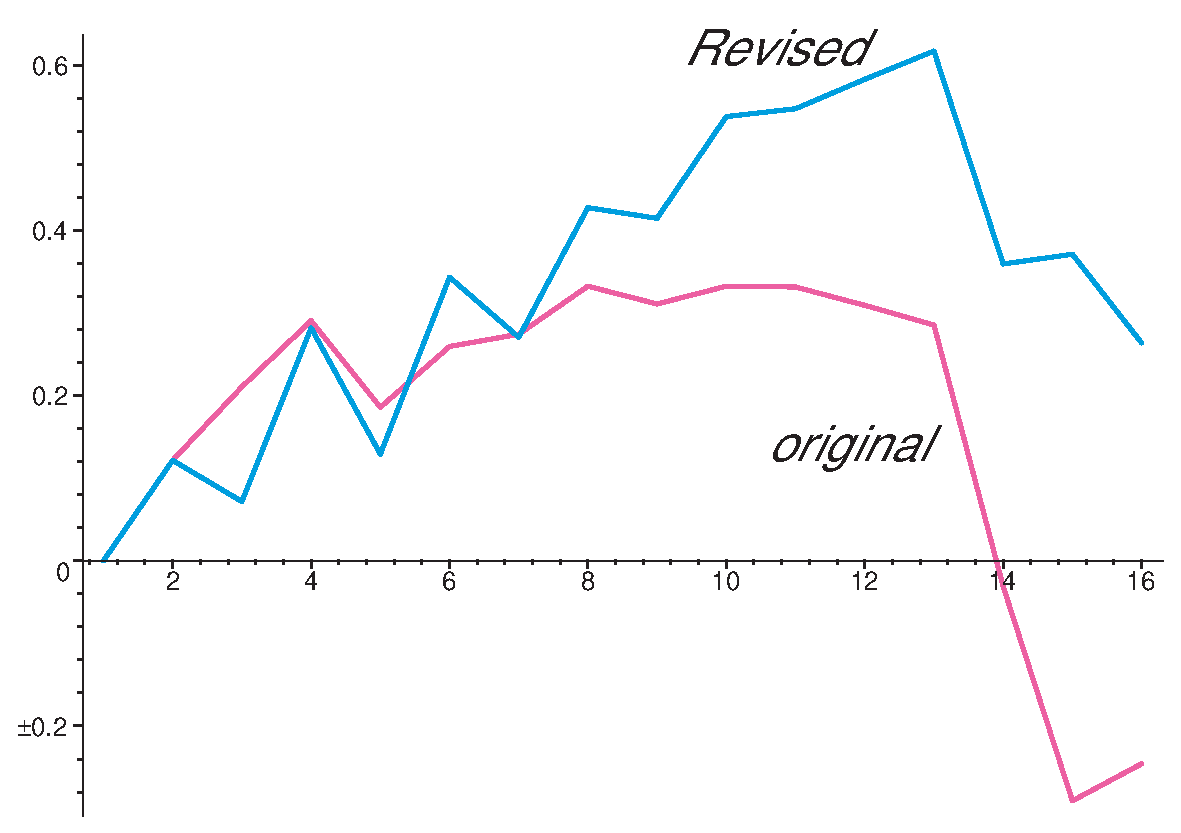
\includegraphics[width=95mm]{./figs/FreeEnergyRev2.eps}
\caption{relaxation後のエンタルピー変化に,並進,回転のエントロピーを精密に求めた場合の自由エネルギーの変化.}
\label{FreeEnergyRev2}
\end{center}\end{figure}

%\fi
\section{まとめ}
Fe-Cu系は構成元素間のサイズ,質量,剛性率にほとんど差がなく,有限温度の振動エントロピーによる影響を無視することが可能である.また,析出クラスターが極めて小さいことから終状態の内部配置エントロピーを無視してもよかろう.このような理想的な系においては,分散した溶質原子がクラスターへ凝集することによる配置エントロピーのロスによって,活性化エネルギーの山が現れていることが明らかとなった.

ここで提案した計算法の特徴は以下の通りである.
\begin{enumerate}
\item 界面エネルギーを求める必要がない,
\item 信頼できる第一原理計算から直接求まる,
\item 核生成の始・終状態を明確に定義している.
\end{enumerate}
より多くの系へこの計算を適用する努力をおこなっている.

\appendix
\section{核生成のkinetic理論}
\cite{BinderStauffer:1976}らが提案したclusterダイナミックスは,古典的なdropletモデルの拡張である.したがって,detailed balanceの議論で出てくるものとおなじクラスターの平衡分布が問題となる.\cite{BeckerDoring:1935}らのクラスターダイナミックスの取り扱いをまとめておく(ここでの記述は主に\cite{Russel:1980}に拠った).

\subsection{Fokker-Planck方程式:平衡分布は動力学でどう使われるか}
クラスターは図\ref{ClusterGrowth}に示したように,一個の原子がくっついたり離れたりするミクロな機構によって成長すると仮定する.時間$t$において原子$n$個を含んだクラスターの濃度を$f(n,t)$とする.$n$個のクラスターが$n+1$のクラスターになる確率を$w(n+1,n)$とすると,$f(n,t)$の時間変化は
\begin{eqnarray}
\frac{\partial f(n,t)}{\partial t} &=& J(n-1) - J(n) \nonumber \\
&=&w(n,n-1)f(n-1,t) - w(n-1,n)f(n,t) \nonumber \\
& &- \left\{w(n+1,n)f(n,t) - w(n,n+1)f(n+1,t) \right\}
\label{dfdt}
\end{eqnarray}
で与えられる.ここで$J(n)$は$n$から$n+1$になるfluxに相当する.
\begin{figure}\begin{center}
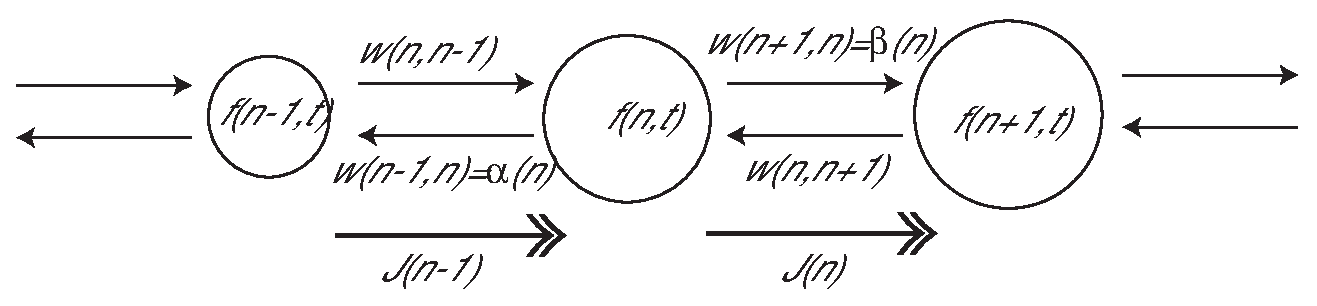
\includegraphics[width=75mm]{./figs/ClusterGrowth.eps}
\caption{クラスターの成長にともなう原子の出入りの確率とフラックス.}
\label{ClusterGrowth}
\end{center}\end{figure}

$w$を原子の捕獲確率$w(n+1,n)=\beta(n)$と放出確率$w(n,n+1)=\alpha(n+1)$とすると,フラックス$J$は
\begin{equation}
J(n) = \beta(n) f(n,t) - \alpha(n+1) f(n+1,t)
\label{Jflux}
\end{equation}
となる.固体の核生成の場合は$\beta$は対象とするクラスターの方向へのジャンプ頻度とn-merへ一回のジャンプで移れる原子の数との積であろう.つまり表面積に比例している.(ほんとかな)vacancyメカニズムだと...

$\alpha$の方はちょっとむづかしい.なぜなら,離脱頻度は析出物表面の結合力によるポテンシャルを感じている原子にとっては,$\beta$で考えたような単純なrandom walkが成り立たないからである.$\alpha$は$J(n)$に値が存在する場合やクラスターが非平衡分布の状態でも,それほど平衡状態と違わないという仮定を置く.平衡状態では,個々のプロセスがそれの逆のプロセスと同じ頻度で起こるとする,詳細釣り合いの原理(the principle of detailed balancing)が成立する.すると\ref{Jflux}式で,$J(n)=0,f(n,t)=C(n)$として
\begin{equation}
\alpha(n+1)=\beta(n) \frac{C(n)}{C(n+1)}
\label{alpha}
\end{equation}
が得られる.この仮定は,n-merクラスターが次の原子が付着するまでに内部緩和を起こす程度の時間があり,他のクラスターと相互作用していないかぎり,成立する.通常は$1/\beta(n)$は内部緩和に比べて十分遅く,クラスターの濃度は非常に小さいため,この仮定は成り立つ.

(\ref{Jflux})式と(\ref{alpha})式とを組み合わせると
\begin{equation}
J(n) = \beta(n) C(n)\left\{
\frac{f(n+1,t)}{C(n+1)} - \frac{f(n,t)}{C(n)} \right\}
\end{equation}
が与えられる.通常の緩やかな変化では微分形に直せて
\begin{equation}
J(n)= -\beta(n)C(n) \frac{\partial f(n,t)/C(n)}{\partial n} .
\label{Jflux2}
\end{equation}
(\ref{dfdt})式に代入すると
\begin{eqnarray}
\frac{\partial f(n,t)}{\partial t} &=& J(n-1) - J(n) \nonumber \\
 &=& -\beta(n-1) C(n-1) \frac{\partial f(n-1,t)/C(n-1)}{\partial n} \nonumber \\
 &+&\beta(n) C(n) \frac{\partial f(n,t)/C(n)}{\partial n} \nonumber \\
 &=&\frac{\partial}{\partial n}\left[
\beta(n) C(n) \frac{\partial f(n,t)/C(n)}{\partial n} \right]
\label{FokkerPlanck}
\end{eqnarray}
となる.最後の変形はここでも微分形に直せるとした.これがクラスター形成の動力学を記述するFokker-Planck方程式である.この式は(\ref{Jflux2})式にガウスの定理(the divergence theorem)をあてはめて直接求めることも可能である.


\subsection{定常状態}
(\ref{Jflux2})式を$J(n)={\rm const} (J_{\rm s})$の下で求める.この場合,すべてのフラックスが一定となる定常状態を意味している.BeckerとD\"{o}ringは次のような境界条件を選定し,時間に依存しない定常解を求めた.
\begin{eqnarray}
& &\frac{f(n)}{C(n)} \rightarrow 1 \ {\rm where} \ n \rightarrow 1 \nonumber \\
& &\frac{f(n)}{C(n)} \rightarrow 0 \ {\rm where} \ n \rightarrow \infty 
\end{eqnarray}
これは$C(n)$の形状から次のように導かれる.クラスターの生成自由エネルギー$\Delta G(n)$がenergy barrierをもち,
\begin{equation}
C(n) = N \exp \left( -\frac{\Delta G(n)}{kT}\right)
\end{equation}
で与えられるとする.ここで係数$N$は単位体積当たりの格子サイトの数で,希薄溶体においてミキシングの部分エントロピーが,n-merのサイズによらず$k \ln(f(n)/N)$で与えられるからである(?).$n$が小さい領域では,クラスターは一原子の孤立した状態へ容易に戻り,平衡状態に近づき$f(n)/C(n)$は1になる.一方,$n$が大きいと$C(n)$はどんどん大きくなるが$f(n)$は有限の値にとどまるので$f(n)/C(n)$は0になる.

すると(\ref{Jflux2})式を変形して積分すると
\begin{equation}
- \int^{0}_{1}{\frac{1}{J_{\rm s}} {\rm d} \left(\frac{f(n)}{C(n)} \right)} =
\int^{\infty}_{1}{\frac{1}{\beta(n)C(n)}{\rm d}n}
\end{equation}
この左辺の積分を実行すると,BeckerとD\"{o}ringの条件から$1/J_{\rm s}$となり,クラスター濃度分布を代入して,
\begin{equation}
J_{\rm s} = \left\{ \int^{\infty}_{1}{\frac{{\rm d}n}{\beta(n)N \exp (-\Delta G(n)/kT)} }
\right\}^{-1}
\end{equation}
が得られる.

この積分は被積分関数$\exp(\Delta G/kT)$の形状特性から一般的に次のようにして求められる.クラスター生成の自由エネルギーを実際に入れると被積分関数のexpの部分$\exp(\Delta G/kT)$は図\ref{dG}に示したような関数となる.$\beta(n)$が十分に緩やかに変化すると仮定すると,critical radiusのまわりを忠実に積分すれば十分な近似と考えられる.そこで$\Delta G(n)$をcritical number $n^*$のまわりで$n$でTaylor展開すると
\begin{equation}
\Delta G(n) = \Delta G(n^*) + \frac{(n-n^*)^2}{2}
\left(\frac{\partial^2 \Delta G}{\partial n^2} \right)_{n^*}
\end{equation}
となる.これを代入して,積分の下限を$-\infty$で置き換えて,ガウス積分
\begin{equation}
\int_{-\infty}^{\infty} \exp(-a x^2) {\rm d} x = \sqrt{\pi/a}
\end{equation}
を用いると,積分結果は
\begin{equation}
J_{\rm s} = Z \beta^* N \exp\left( - \frac{\Delta G^*}{kT} \right)
\end{equation}
ここで,$Z$はZeldovich因子で,
\begin{equation}
Z = \sqrt{-\frac{1}{2\pi kT} 
\left(\frac{\partial^2 \Delta G}{\partial n^2}\right)_{n=n^*}}
\end{equation}
で与えられる.
\begin{figure}\begin{center}
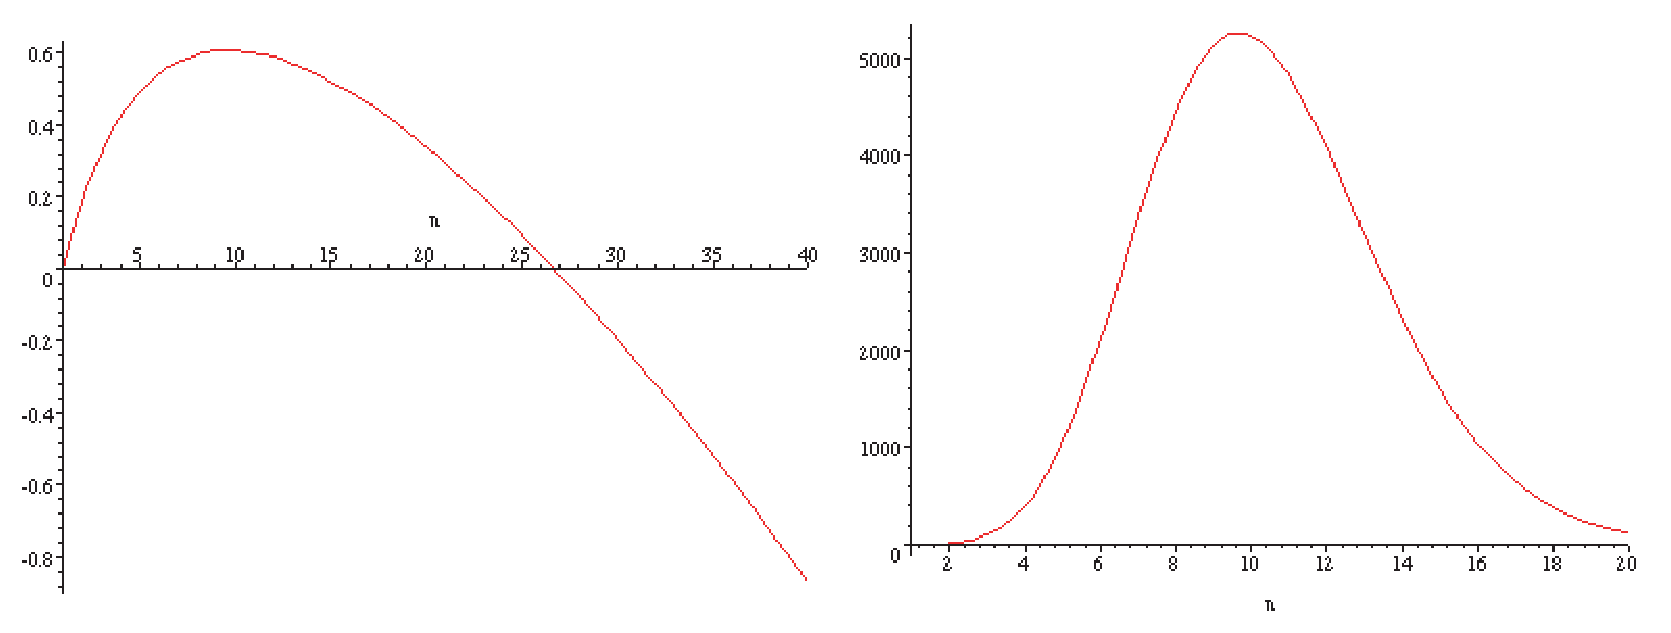
\includegraphics[width=125mm]{./figs/dG.eps}
\caption{クラスター生成の自由エネルギー$\Delta G(n)$と被積分関数$\exp(\Delta G/kT)$.}
\label{dG}
\end{center}\end{figure}

このZeldvichの導き方は一見正しそうに見える.しかし,固体からの析出のように臨界核が非常に小さい場合,$\beta(n)$に含まれる界面の面積変化も含めるとTaylor展開が妥当かどうかは不明である.$Z=10^{-2}$という非常に小さな値である通常の場合と違うので,数値計算で比較する必要がある.

\subsection{潜伏時間}
潜伏期間はFokker-Planck方程式(\ref{FokkerPlanck})の解を求めて,定常核生成状態に移るまでの期間をとる.一般的にはこのような遷移期間はexp関数で近似できて,
\begin{equation}
J(t) = J_{\rm s} \exp(-\tau/t)
\end{equation}
で求めら,この$\tau$を潜伏期間としている.正確な解析解は違うがそちらが正しいかどうかは???

ここではFederらの取り扱いを解説した榎本の記述を転記する.Federらは核生成理論が大前提としている,(II)揺らぎによる生成,消滅過程が平均的におなじ過程で起こる,(III)マクロな法則に従うという二つの仮定をつかってFokker-Planck方程式が記述している物理現象を解析した.(\ref{FokkerPlanck})式の内側の微分を実行すると
\begin{equation}
\frac {\partial}{\partial n}\left(\frac{f(n,t)}{C(n)}\right) =
\frac{\frac{\partial}{\partial n}f(n,t)}{C(n)}-
\frac{f(n,t) \frac{\partial C(n)}{\partial n}}{ C(n)^{2}}
\end{equation}
となる.これを代入すると
\begin{eqnarray}
\frac{\partial f(n,t)}{\partial t}
&=&\frac{\partial}{\partial n}\beta(n) C(n)\left(
\frac{\frac{\partial}{\partial n}f(n,t)}{C(n)}-
\frac{f(n,t) \frac{\partial C(n)}{\partial n}}{ C(n)^{2}}
\right) \nonumber \\
&=&\frac{\partial}{\partial n}
\left( \beta(n) \frac{\partial f (n,t)}{\partial n} - 
\frac{\beta(n)}{C(n)} f(n,t) \frac{\partial C(n)}{\partial n}
\right) \nonumber \\
&=&\frac{\partial}{\partial n}
\left( \beta(n) \frac{\partial f (n,t)}{\partial n} \right)
-\frac{\partial}{\partial n}
\left( \beta(n) f (n,t) \frac{\partial \ln C(n)}{\partial n} \right)
 \nonumber \\
&=&\frac{\partial}{\partial n}
\left( \beta(n) \frac{\partial f (n,t)}{\partial n} \right)
+ \frac{\partial}{\partial n}
\left( \frac{\beta(n) f (n,t)}{kT} \frac{\partial \Delta G(n)}{\partial n} \right)
\end{eqnarray}
となる.最後の変形には
\begin{equation}
\frac{\partial}{\partial n} \ln C(n) =
-\frac{1}{kT} \frac{\partial \Delta G(n)}{\partial n}
\end{equation}
を用いた.

右辺の第1項は拡散,第2項はそれに対するポテンシャル勾配の影響を表す.$n$の小さい領域では$\Delta G(n)$の$n$に対する勾配が大きく,第2項が効いて,クラスターは素早く成長,分解する.$n \sim n^*$付近ではポテンシャル勾配が小さくなるため第1項が支配的となる.この領域では原子が付着と離脱を繰り返すので成長が遅く,ここを通過する時間が定常拡散へいくまでの時間の大部分を占めていると考えてよい.

揺らぎの領域を$\Delta G^*$から幅$\sim kT$以内とし,対応するクラスター分布の幅を$\delta$とすると
\begin{equation}
\delta =\left\{- \frac{1}{8kT} 
\left. \frac{\partial^2 \Delta G(n)}{\partial n^2} \right|_{n^*} 
\right\}^{-1/2}
\end{equation}
となる.$\beta(n)$には表面積が含まれているがその変化は小さいとして臨界核での$\beta^*$を拡散係数とすると,$\delta \sim \sqrt{\beta^* \tau}$と書けるから,
\begin{equation}
\tau \sim -\frac{\chi  k T}{\beta^* \left. \frac{\partial^2 \Delta G(n)}{\partial n^2} \right|_{n^*}  }
\end{equation}
ここで,$\chi$は8であるが,Federらは4とした.Zeldovich係数を使うと
\begin{equation}
Z^2 = - \frac{1}{6.28 kT} \left. \frac{\partial^2 \Delta G(n)}{\partial n^2} \right|_{n^*} 
\end{equation}
であるので,$\delta \sim Z^{-1}$.よって$\chi =4$とすると
\begin{equation}
\tau = \frac{1}{2 Z^2 \beta^*}
\end{equation}
と近似できる.この結果は数値的にFokker-Planck方程式を解いた結果と一致している.これも確認する必要がある.

\section{核生成の系のgrand partition function}
droplet modelのgrand partition functionに関する解説で,もっとも簡単な形で示した\cite{Kastrup:1998}の記述にしたがって表記する.
$n$個の構成原子(constituents)で構成されたdropletsを考える.系の次元を$d \leq 2$とすると,過剰エネルギー(多分自由エネルギー)$\epsilon_n$は
\begin{equation}
\epsilon_n = - \hat{\mu} n - \sigma n^{1-1/d} 
\end{equation}
で与えられる.ここで第一項は体積に比例する項,第二項は表面エネルギーに相当する項である.磁場中のIsing spin模型では磁場を$H$とすると$\hat{\mu} = -2H$.過飽和ガスからのdropletの生成では$\hat{\mu} = \mu -\mu_c$で,$\mu$および$\mu_c$はそれぞれ化学ポテンシャルと凝縮点での臨界化学ポテンシャルを示す.Fisherが指摘しているような$\ln n$に比例する項は無視している.

平均のdroplet数$\bar{\nu}(n)$がBoltzmann因子で与えられ
\begin{equation}
\bar{\nu}(n) \propto \exp{-\beta \epsilon_n}, \beta=\frac{1}{k_{\rm B}T},
\end{equation}
そしてdropletはお互いが相互作用しない希薄気体をつくると仮定すると,スピンあたりあるいは体積あたりのthe grand canonical potential $\Psi_d$が以下のように導かれる.
\begin{eqnarray}
\Psi_d(\beta, t) = \ln Z_G = p \beta &=&
 \sum_{n=0}^{\infty}\exp\left(\beta \hat{\mu} n-\beta\sigma n^{1-1/d}\right) \\ 
t=\beta \hat{\mu}, x&=&\beta \sigma, p:\textrm{pressure} \nonumber \\
d \Psi_d &=& - U d\beta + \bar{n} dt
\end{eqnarray}

この級数は$t \leq 0$の時のみ,Maclaurin-Cauchy integral criteriumにより,収束する.ところが,実際には$t \geq 0$の準安定領域での$\Psi_d$の振る舞いに興味が持たれるところである.これがLangerが示した解析接続の理論であるが,Penroseが示したところによると,数学的な厳密さを欠いたものであったようである.

この級数を,$n$を連続変数に変えて積分形にしてみよう.$t < 0$で
\begin{equation}
\overline {\psi _d}=\int_0^\infty  {\exp \beta \left( {\hat \mu n-\sigma n^{1-1/d}} \right)\textrm{d}n}
\end{equation}
さらに$n=\left( {{\sigma  \mathord{\left/ {\vphantom {\sigma  {\hat \mu }}} \right. \kern-\nulldelimiterspace} {\hat \mu }}} \right)^d u^d$
で変数変換すると
\begin{eqnarray}
\overline {\psi _d}=d\left( {{\sigma  \over {\hat \mu }}} \right)^d\int_0^\infty  {u^{d-1}\exp \beta h\left( u \right)\textrm{d}u}
\\
h\left( u \right)=a\left( {u^d-u^{d-1}} \right),a={{\sigma ^d} \over {\hat \mu ^{d-1}}}. \nonumber
\end{eqnarray}
関数$h(u)$は$u=u_0=0$と$u=u_1=1-1/d$に極値を持つ.一般的な解析に従うと大きな$\beta$に対して上の積分は近似(漸近展開:the asymptotic expansion)されて
\begin{equation}
\overline {\psi _d}\sim \left( {1-{1 \over d}} \right)^{{d \mathord{\left/ {\vphantom {d 2}} \right. \kern-\nulldelimiterspace} 2}}\sqrt {{{\pi d} \over {2\beta \hat \mu }}}\left( {{\sigma  \over {\hat \mu }}} \right)^{{d \mathord{\left/ {\vphantom {d 2}} \right. \kern-\nulldelimiterspace} 2}}\exp \left( {-{{\beta a} \over d}\left( {1-1/d} \right)^{d-1}} \right)\left[ {i+O\left( {1/\beta } \right)} \right]
\end{equation}
を得る.ここで複素$u$平面の経路は$u_0$から$u_1$をとおり,その後複素数軸にそって$+i\infty$まで向っている.したがって,最急降下に添った関連するガウス積分の片側のみが寄与する.支配的な項は純粋に複素数である.

さらにLangerは自由エネルギーの虚数部が核生成の頻度を表すことを導き(Langer and Schwart),これはKampmann and Wagnerへつながっているらしい.

\section{Beckerの界面モデル}
A-B2元合金で$\alpha$相と$\beta$相が界面を形成しているとする.この界面を横切る結合エネルギーの総和を$E_{\alpha \beta}$,$\alpha$相と$\beta$相の内部で界面と平行な面を横切る結合のエネルギーの総和を$E_{\alpha \alpha}$および$E_{\beta \beta}$とすると界面エネルギーは
\begin{equation}
\sigma = E_{\alpha \beta} - 
\frac{1}{2} \left(E_{\alpha \alpha}+E_{\beta \beta} \right)
\end{equation}
によって計算される.

\begin{maplegroup}
\begin{mapleinput}
\mapleinline{active}{1d}{EE:=(xa,xb)->NsZs*((1-xa)*(1-xb)*eaa+xa*xb*ebb+(xa*(1-xb)+(1-xa)*xb)*
eab);}{%
}
\end{mapleinput}

\mapleresult
\begin{maplelatex}
\mapleinline{inert}{2d}{EE := proc (xa, xb) options operator, arrow;
NsZs*((1-xa)*(1-xb)*eaa+xa*xb*ebb+(xa*(1-xb)+(1-xa)*xb)*eab) end
proc;}{%
\maplemultiline{
\mathit{EE} := (\mathit{xa}, \,\mathit{xb})\rightarrow  \\
\mathit{NsZs}\,((1 - \mathit{xa})\,(1 - \mathit{xb})\,\mathit{eaa
} + \mathit{xa}\,\mathit{xb}\,\mathit{ebb} + (\mathit{xa}\,(1 - 
\mathit{xb}) + (1 - \mathit{xa})\,\mathit{xb})\,\mathit{eab}) }
%
}
\end{maplelatex}

\end{maplegroup}
\begin{maplegroup}
\begin{mapleinput}
\mapleinline{active}{1d}{sigma:=EE(xa,xb)-(EE(xa,xa)+EE(xb,xb))/2;}{%
}
\end{mapleinput}

\mapleresult
\begin{maplelatex}
\mapleinline{inert}{2d}{sigma :=
NsZs*((1-xa)*(1-xb)*eaa+xa*xb*ebb+(xa*(1-xb)+(1-xa)*xb)*eab)-1/2*NsZs*
((1-xa)^2*eaa+xa^2*ebb+2*xa*(1-xa)*eab)-1/2*NsZs*((1-xb)^2*eaa+xb^2*eb
b+2*xb*(1-xb)*eab);}{%
\maplemultiline{
\sigma  := \mathit{NsZs}\,((1 - \mathit{xa})\,(1 - \mathit{xb})\,
\mathit{eaa} + \mathit{xa}\,\mathit{xb}\,\mathit{ebb} + (\mathit{
xa}\,(1 - \mathit{xb}) + (1 - \mathit{xa})\,\mathit{xb})\,
\mathit{eab}) \\
\mbox{} - {\displaystyle \frac {1}{2}} \,\mathit{NsZs}\,((1 - 
\mathit{xa})^{2}\,\mathit{eaa} + \mathit{xa}^{2}\,\mathit{ebb} + 
2\,\mathit{xa}\,(1 - \mathit{xa})\,\mathit{eab}) \\
\mbox{} - {\displaystyle \frac {1}{2}} \,\mathit{NsZs}\,((1 - 
\mathit{xb})^{2}\,\mathit{eaa} + \mathit{xb}^{2}\,\mathit{ebb} + 
2\,\mathit{xb}\,(1 - \mathit{xb})\,\mathit{eab}) }
%
}
\end{maplelatex}

\end{maplegroup}
\begin{maplegroup}
\begin{mapleinput}
\mapleinline{active}{1d}{factor(collect(collect(collect(expand(sigma),eaa),ebb),eab));}{%
}
\end{mapleinput}

\mapleresult
\begin{maplelatex}
\mapleinline{inert}{2d}{-1/2*NsZs*(xa-xb)^2*(-2*eab+eaa+ebb);}{%
\[
 - {\displaystyle \frac {1}{2}} \,\mathit{NsZs}\,(\mathit{xa} - 
\mathit{xb})^{2}\,( - 2\,\mathit{eab} + \mathit{eaa} + \mathit{
ebb})
\]
%
}
\end{maplelatex}

\end{maplegroup}

\bibliographystyle{apalike}
\bibliography{Nucleation_Background}
\end{document}

